\documentclass[12pt]{article}
\usepackage[T1]{fontenc}
\usepackage[utf8]{inputenc}
\usepackage{url}
\usepackage{enumerate}
\usepackage[top=3cm, bottom=3cm]{geometry}
\usepackage{graphicx} 
\usepackage{enumitem}
\usepackage{natbib}
\usepackage{listings}
\usepackage{float}
\usepackage{amsmath}
\usepackage{color}
\bibpunct{[}{]}{,}{a}{}{;}
\setcitestyle{super}

% Variables
\newcommand{\assignmentname}{Assignment 3}
\newcommand{\coursename}{Statistical Methods in Machine Learning}
\newcommand{\studentnameOne}{Bjarki Madsen (lch929)}
\newcommand{\studentnameTwo}{Disha Singh (cfn492)}
\newcommand{\studentnameThree}{Sokratis Siozos - Drosos (dnb823)}
\newcommand{\department}{Department of Computer Science}
\newcommand{\institution}{Copenhagen University}
\newcommand{\location}{Copenhagen, Denmark}

\begin{document}

\renewcommand\refname{References}

\title{\assignmentname \\ {\Large {\textsc \coursename}}}
\author{
        \studentnameOne \\
        \studentnameTwo \\
        \studentnameThree \\ \\
                \department \\
        \institution \\
        \location
}
\date{\today}

\maketitle
\thispagestyle{empty}

\pagebreak

\section*{II.1 Neural Networks}

  \subsection*{III.1.1 Neural network implementation}

    \subsubsection*{Finding the derivative}

      Given the activation function:
        $$h(a) = \frac{a}{1 + |a|} \\$$
      we calculate the derivative by using the quotient rule:
        $$\frac{d}{dx}f(x) = \frac{\frac{d}{dx}g(x)h(x) - g(x)\frac{d}{dx}h(x)}{(h(x))^2}$$
      where we set $g(x) = a$ and $h(x) = 1 + |a|$. That gives:
        \begin{align*}
          \frac{d}{da}f(a) &= \frac{\frac{d}{da}a(1+|a|) - a(\frac{d}{da}(1 + |a|)}{(1+|a|)^2} \\
          &= \frac{(1 + |a|) - a\frac{a}{|a|}}{(1+|a|)^2} \\
          &= \frac{1 + |a| - \frac{a^2}{|a|}}{(1+|a|)^2} \\
        \end{align*}
      Since $\frac{a^2}{|a|}$ is simply $a$, where $a > 0$, subtracting $|a|$ from $a$ gives zero and therefore we get:
        $$\frac{d}{da}f(a) = \frac{1}{(1+|a|)^2}$$

    \subsubsection*{Neural Network implementation}

      Our implementation is in the class \texttt{Neural\_Network} in \texttt{NN\_.py}.

  \subsection*{III.1.2 Neural network training}

    Sadly, this part of the assignment was not completed. Our implementation of the network is not easily trainable and we expect our implementation to be the cause of that, mainly the backpropagation. However, when we apply the gradient descent we \textit{are} able to get the MSE cost down, usually to around 1. Still, we think that this cost is way to high and therefore we don't get our expected results.

    As figure \ref{figure:predictions} and \ref{figure:predictions2} clearly show, our network is lacking some fundamental property that we could not figure out in time.

    \begin{figure}[h]
      \centering
      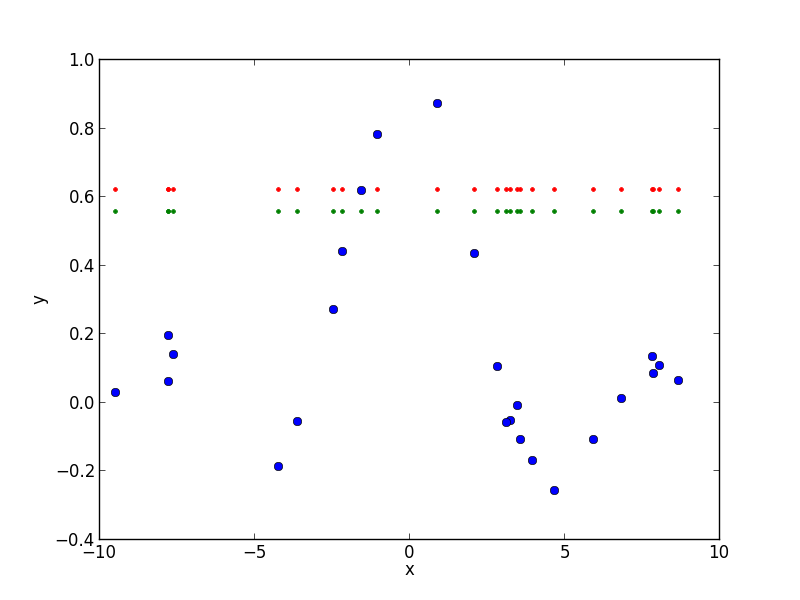
\includegraphics[width =1\textwidth]{figures/predictions.png}
      \caption{Prediction for training data.}
      \label{figure:predictions}
    \end{figure}

    \begin{figure}[h]
      \centering
      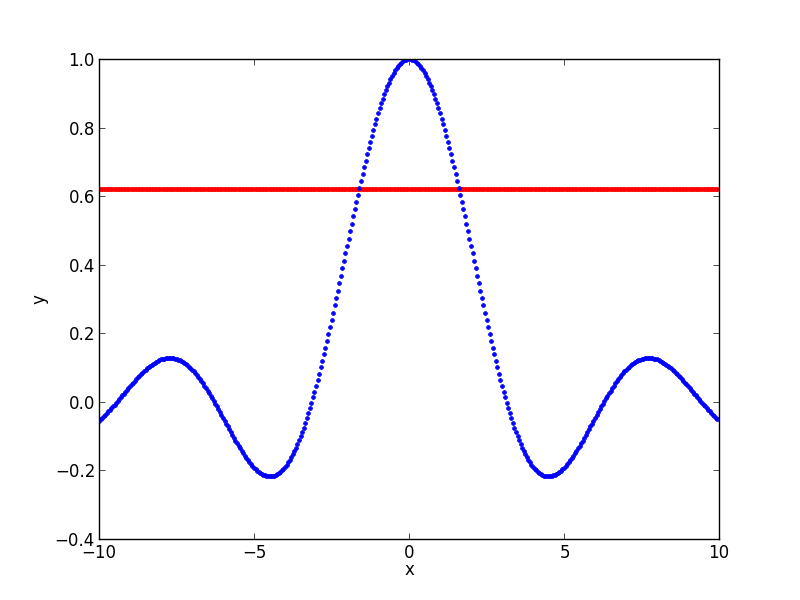
\includegraphics[width =1\textwidth]{figures/function1_1_and_prediction.png}
      \caption{The predictions for the sampled sinc function.}
      \label{figure:predictions2}
    \end{figure}




\section*{III.2 Support Vector Machines}

  \subsection*{III.2.1 Data normalization}

    \begin{table}[h]
      \begin{tabular}{l|l|l|l|l|}
      \cline{2-5}
                                        & Train Mean    & Test Mean     & Train Variance & Test Variance \\ \hline
      \multicolumn{1}{|l|}{Feature 1}   & 155.960       & -0.079        & 1962.809       & 0.732         \\ \hline
      \multicolumn{1}{|l|}{Feature 2}   & 204.821       & -0.158        & 9633.816       & 0.715         \\ \hline
      \multicolumn{1}{|l|}{Feature 3}   & 115.059       & 0.056         & 2093.574       & 0.798         \\ \hline                         
      \multicolumn{1}{|l|}{Feature 4}   & 0.006         & 0.113         & 0.000          & 1.990         \\ \hline                         
      \multicolumn{1}{|l|}{Feature 5}   & 0.000         & 0.072         & 0.000          & 1.666         \\ \hline                         
      \multicolumn{1}{|l|}{Feature 6}   & 0.003         & 0.087         & 0.000          & 2.137         \\ \hline                         
      \multicolumn{1}{|l|}{Feature 7}   & 0.003         & 0.116         & 0.000          & 1.922         \\ \hline                         
      \multicolumn{1}{|l|}{Feature 8}   & 0.010         & 0.087         & 0.000          & 2.138         \\ \hline                         
      \multicolumn{1}{|l|}{Feature 9}   & 0.028         & 0.249         & 0.000          & 1.772         \\ \hline                         
      \multicolumn{1}{|l|}{Feature 10}  & 0.262         & 0.245         & 0.026          & 1.829         \\ \hline                         
      \multicolumn{1}{|l|}{Feature 11}  & 0.015         & 0.230         & 0.000          & 1.717         \\ \hline                         
      \multicolumn{1}{|l|}{Feature 12}  & 0.017         & 0.251         & 0.000          & 1.778         \\ \hline                         
      \multicolumn{1}{|l|}{Feature 13}  & 0.022         & 0.317         & 0.000          & 2.190         \\ \hline                         
      \multicolumn{1}{|l|}{Feature 14}  & 0.044         & 0.230         & 0.001          & 1.717         \\ \hline                         
      \multicolumn{1}{|l|}{Feature 15}  & 0.023         & 0.149         & 0.001          & 2.663         \\ \hline                         
      \multicolumn{1}{|l|}{Feature 16}  & 22.001        & -0.057        & 16.510         & 1.361         \\ \hline                         
      \multicolumn{1}{|l|}{Feature 17}  & 0.495         & 0.074         & 0.010          & 1.083         \\ \hline                         
      \multicolumn{1}{|l|}{Feature 18}  & 0.716         & 0.087         & 0.003          & 0.951         \\ \hline                         
      \multicolumn{1}{|l|}{Feature 19}  & -5.764        & 0.155         & 1.062          & 1.217         \\ \hline                         
      \multicolumn{1}{|l|}{Feature 20}  & 0.215         & 0.311         & 0.006          & 1.363         \\ \hline                         
      \multicolumn{1}{|l|}{Feature 21}  & 2.366         & 0.087         & 0.136          & 1.134         \\ \hline                         
      \multicolumn{1}{|l|}{Feature 22}  & 0.200         & 0.169         & 0.007          & 1.415         \\ \hline
      \end{tabular}
      \caption{Mean and variance for training data and normalized test data.}
      \label{table:mean_var_train_norm_test}
    \end{table}

  \subsection*{III.2.2 Model selection using grid-search}
    For the purpose of this part of the assignment we used the library \texttt{LIBSVM}, which provides the necessary tools to train a model, validate it based on the train data with k-fold validation and predict based on a test file. In addition there are various Python files with utilities like grid-search. 
 

    In order to determine the appropriate SVM hyperparameters we use \texttt{grid.py} from \texttt{LIBSVM} which calculates the best $\gamma$ and $C$ combinations for the minimum $0-1$ loss. 
 

    First, we perform the grid-search on the training data to find the best $\gamma$ and $C$ combination. Once we got that, we performed a 5-fold cross validation on the train set with the $\gamma$ and $C$ that we got. Once we performed the cross validation we trained the model again on the whole training set and applied it on the test set. Table \ref{table:accuracies} shows the accuracy we got in each data set along with the $\gamma$ and $C$ that we used (\textit{Note, the  $\gamma$ value $0.002$, is rounded from $0.001953125$ which we actually used but could not fit in table \ref{table:accuracies}}).
    \begin{table}[h]
      \centering
      \begin{tabular}{|c|c|c|c|} \hline
      & Validation &  Test  & $C, \gamma $\\ \hline
      Raw data  & $87.7551\%$ &  $86.5979\% (84/97)$& $8.0, 0.002$ \\ \hline
      Normalized data & $91,8367\%$ & 89.6907\% (87/97) & $8.0, 0.125$\\ \hline
      \end{tabular}
      \caption{Accuracy of the SVM on both raw and normalized data for 5-fold cross validation and testing}      
      \label{table:accuracies}
    \end{table}

    As it can be observed from table \ref{table:accuracies}, data normalization improved the accuracy of the SVM on both validation and testing.
    
  \subsection*{III.2.3 Inspecting the kernel expansion}

    \subsubsection*{III.2.3.1 Support vectors}

      In the SVM Model, C controls the cost of misclassification on the training data. The goal of SVM is to find a hyperplane that would leave the widest possible margin between input points from two classes. In large number of dimensions, training data can often be explained quite well by overfitting the model. Drastically small C makes the cost of misclassification low, known as a \textit{soft margin}, thus allowing more of them for the sake of wider margin. Drastically large C makes the cost of misclassification high, \textit{hard margin}, thus forcing the algorithm to explain the input data stricter and with potential overfit. This can be observed in figure \ref{figure:SV}

      \begin{figure}[h]
        \centering
        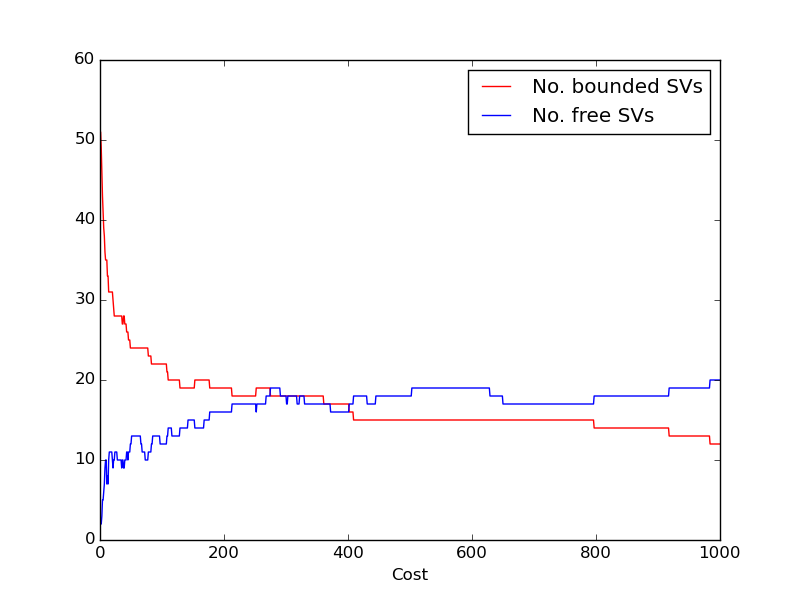
\includegraphics[width =1\textwidth]{figures/SVplot.png}
        \caption{Changes in number of bounded and free Support Vectors based on cost variation}
        \label{figure:SV}
      \end{figure}

      \subsubsection*{III.2.3.2 Scaling behavior}

        The effect of data on SVMs is in direct relation. If we increase the data, it will increase the number of support vectors. This results in increase in cost as well as precision. Increasing the number of training patterns and increasing C will reduce the amount of support vectors.

\end{document}
% End of document.







